\documentclass[11pt,onecolumn]{article} 

\usepackage{latex8}
\bibliographystyle{latex8}

\usepackage{times}

% for highlighting todos and fixes
\usepackage{color, soul}

% for figures
\usepackage{caption}
\usepackage{graphicx}

\usepackage{amsmath}
\usepackage{setspace}

% for references and urls
\usepackage{url}
%\usepackage{hyperref} % we can use this, but it makes a weird table of contents with the formatting we are using

\newcommand{\h}[1]{\hl{#1}}
\newcommand{\specialcell}[2][c]{%
  \begin{tabular}[#1]{@{}l@{}}#2\end{tabular}}

\singlespacing	% we can bump this to \onehalfspacing to increase readability if you want

\begin{document}

\title{Clever Title}

\author{
 Aaron Stacy \\ \and
 Calvin MacKenzie \\
}

\maketitle

\Section{Introduction}

Originally developed by Andrew Viterbi to decode signals over noisy channels, the Viterbi algorithm proved to be useful in a wide variety of areas. Within the field of Natural Language Processing (NLP), the Viterbi algorithm is most commonly used with Hidden Markov Models (HMM) to find the most likely sequence of part-of-speech tags, and other related tagging tasks.

Closely related to the Viterbi algorithm is the Forward algorithm, which is used within NLP to efficiently compute observation likelihood. While not as popular as the Viterbi algorithm, the Forward algorithm is a fundamental algorithm within NLP. The implementations of the two algorithms are actually quite similar and they share the same running time of $O(T N^2)$.

Work on improving the Viterbi algorithm typically comes from the realm of signal processing, rather than NLP, where these gains greatly help with the decoding of signals. Typically, these improvements deal with a hardware viterbi decoder and ways to modify this hardware in order to enhance the parallelization of the decoding problem.

Rather than approaching this task from a hardware perspective, we wanted to improve these algorithms with parallelization techniques. We implemented a parallel version of the Viterbi and Forward algorithms using the OpenMP API \footnote{\url{http://openmp.org/wp/}} and characterized the performance over a range of workloads. We tested this on the Wall Street Journal dataset from the Penn Treebank and varied the size of the dataset to measure performance. We ran the algorithm on the TACC cluster in order to find strong and weak scaling characteristics.

\Section{Related Work}

\begin{figure}[h!]
\centering
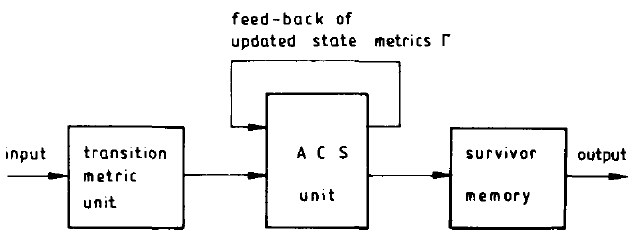
\includegraphics[width=.5\linewidth]{figures/pipeline}
\caption{Pipeline structure of Viterbi decoder}
\label{fig:pipeline}
\end{figure}

The work by Fettweis and Meyr (1989) \cite{acs:old} describes a successful attempt at parallelizing a key bottleneck of the Viterbi algorithm: the add-compare-select component. The authors describe the process of obtaining the updated state metric, $\Gamma_{n+1,z_{i}}$, as the add-compare-select (ACS) unit of the Viterbi algorithm, shown in Figure \ref{fig:pipeline}. The formula to find this updated state is shown below (where $\lambda$ is the transition probability):

\begin{equation}
\Gamma_{n+1,z_{i}} = \max\limits_{\text{all possible } z_{k}\rightarrow z_{i}} (\Gamma_{n,z_{k}} + \lambda_{n,z_{k}\rightarrow z_{i}})
\end{equation}

This equation is at the heart of the Viterbi algorithm, and forces the current state to depend on all previous states with its recursive nature. 

Even though the ACS unit is only one component of the Viterbi algorithm, the authors explain that ``since the ACS unit is much more complex, it is the bottleneck which limits the throughput rate.'' To combat this, the authors introduce the concept of an $M$-step trellis, as opposed to the traditional 1-step trellis used in the Viterbi algorithm. This can be used in the ACS loop, but will take $M$ times as long. Utilizing a combination of the original 1-step trellis and the $M$-step trellis allows the authors to parallelize the Viterbi algorithm in combination with a multiplexer.

\begin{figure}[h!]
\centering
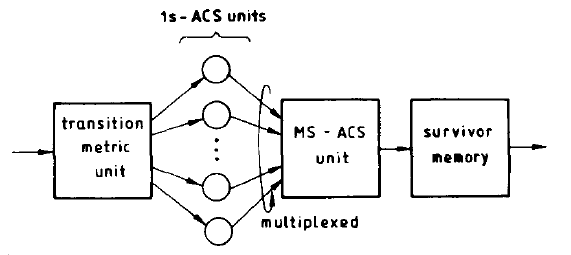
\includegraphics[width=.5\linewidth]{figures/pipeline_multiplex}
\caption{Multiplexed structure of Viterbi decoder}
\label{fig:pipeline_multiplex}
\end{figure}

The new pipeline structure is shown in Figure \ref{fig:pipeline_multiplex}. This is implemented in hardware using a systolic array, which is a pipelined structure of processing units called cells. Each of these cells can be computing in parallel and combined at the end, speeding up the overall process.\\

Du et al. \cite{gatech:bio} proposed extensions to two known methods for parallelizing the computationally intensive kernel of the Viterbi algorithm. The paper is applied to computational biology, so the authors first investigate existing parallelization methods for related sequence alignment algorithms.

The authors also demonstrate how to divide the Viterbi algorithm into two parts: independent sections of the calculation do not depend on previous results, and are therefore more amenable to parallelization. By isolating the dependent ant parts of the computation, the sequential work is minimized and the authors achieve greater speedup.

Because of the difference in application domain, the specifics of the approach taken by Bader et al. cannot be directly applied to NLP. However when designing parallel algorithms the basic principles of locality always apply. There are two specific techniques used by Bader et al. that can be applied to a more general Viterbi algorithm: dividing dependent and independent calculations and streaming algorithms that overlap data transfer with calculation. We were able to use the latter in our implementation.

\Section{Method Overview}

Before implementing any of the algorithms, we first wrote a preprocessor to format the Penn Treebank data. Initially, the Penn Treebank files contained \texttt{<word>/<label>} pairs on each line and this format was not suitable for us. The preprocessor we implemented removed the irrelevant information and each output line contained a sentence of \texttt{<word>/<label>} pairs. An example is shown in Table \ref{table:preprocess}. Our preprocessor also split the data up into multiple sections which helped later on during parallelization.

\begin{figure}
\centering
\begin{tabular}{c c l}
List/VB & $\rightarrow$ & List/VB \\
$[$ the/DT flights/NNS $]$ & $\rightarrow$ & \specialcell{the/DT\\flights/NNS} \\
from/IN & $\rightarrow$ & from/IN \\
$[$ Baltimore/NNP $]$ & $\rightarrow$ & Baltimore/NNP \\
\end{tabular}
\caption{Example of preprocessor converting Penn Treebank files}
\label{table:preprocess}
\end{figure}

\SubSection{Sequential}

Next, we needed to implement sequential versions of the two algorithms. From their definitions, the implementations of the Viterbi and Forward algorithms were straightforward. Since we were not concerned with the resulting scores from the algorithms, we did not construct the probability distribution from the training set, but rather used a random value for the probability of each transition, $P(t_{i}|t_{i-1})$, and emission, $P(w_i|t_i)$. However, we did use the actual words and tags from the dataset.

\SubSection{Parallelization}

Using OpenMP, we were able to add parallelization to the sequential algorithms we had written. In addition, to achieve scalability beyond the limits of memory afforded by the system, the algorithms needed to divide the work into tractable chunks and process them incrementally by bringing a chunk into memory, processing it, and then either writing it out or reducing it, depending on the calculating. We utilized parallelization to overlap the I/O work with computation. 

This parallelization allowed us to explore possible speedups by reading data and allocating the lattice in parallel with applying the Viterbi algorithm. In other words, while on thread or process is reading data from disk, the other can run the algorithm.

We initially set out to explore three levels of parallelism:

\begin{enumerate}
  \item Our most coarse-grained parallelism is simply processing different sentences in parallel. For the most part, this classifies as ``embarassingly parallel,'' since there is no coordination needed between the threads as they process the data. The only coordination required at the end of the forward algorithm is multiplying all of the results to get the full observation probability, which can be accomplished with a strait-forward parallel reduction.

  \item Our fine-grained parallelism involves parallelizing within the Viterbi and forward algorithms. Each time step involves an $O(n^2)$ calculation that is essentially a matrix-vector multiplication (with a unit vector).

\item The final level of parallelism that we explored but did not implement involved parallelizing across time steps of the forward algorithm. Recall that each step involves the recursion, where $v$ refers to the forward lattice, $t$ the time step, $j$ the current state, $n$ the number of states, $b$ the observation probability, and $a$ the transition probability:

  \begin{equation}
    v_{t,j} = b_j(t) \sum_{k=0}^n v_{t - 1, k} a_{k,j}
  \end{equation}

  We were hoping to be able to modify this such that we could calculate the values of the lattice with a parallel prefix sum, however the recursion is exponential not linear (there is a factor of $n$ steps at each of the $t$ iterations), so we could not find a way to do this.

\end{enumerate}

\Section{Experimental Evaluation}

We evaluated our implementation on the Wall Street Journal section of the Penn Treebank, which has 45,920 sentences and 1,107,365 part-of-speech tagged words.

We ran the algorithm on the Lonestar section of the Texas Advanced Computing Cluster (TACC)\footnote{\url{https://www.tacc.utexas.edu/resources/hpc/lonestar}}. These machines run compute nodes with two sockets each, each socket containing six cores, giving each process up to 12 simultaneous processors.

\SubSection{Methodology}

Since our implementation had two levels of parallelism, coarse grained and fine grained, we characterized performance from a single thread at each level up to 12. We did not look at more than a total of 12 threads, though, since the computation is not I/O bound and running more than a total of 12 threads degrades.

We ran the implementation over 5\%, 10\%, and 20\% of the full dataset when determining scaling, and against the full dataset to determine peak performance.

We compared performance of the GNU and Intel compilers.

\SubSection{Results}

We acheived relatively good scaling as shown in the strong scaling plot, Figure ~\ref{fig:strong_scaling}. While the speedup is not perfect, we are able to maintain performance increases as we increase threads all the way up to the cores available on the machine. Note that in the scaling figures the number of threads is the total number of both coarse and fine-grained threads. The scaling plots report the best performing of the thread combinations.

\begin{figure}[h!]
\centering
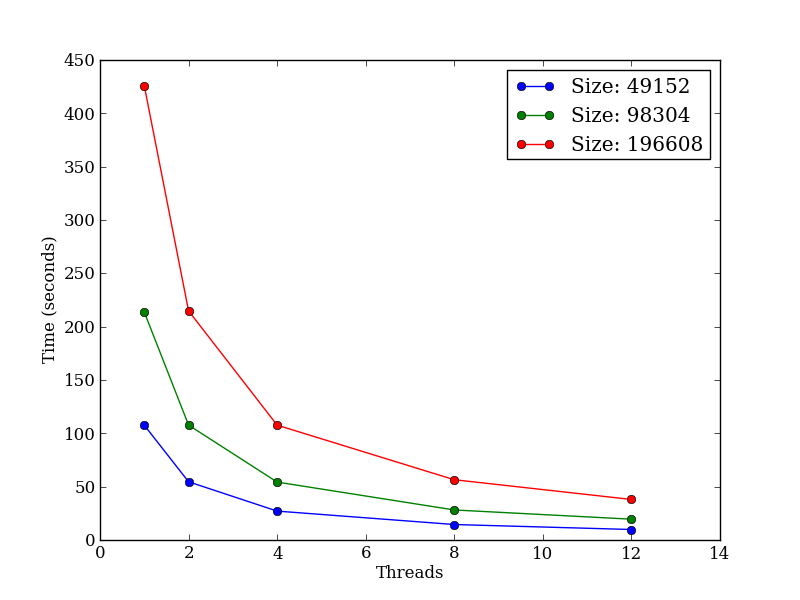
\includegraphics[width=.75\linewidth]{figures/intel_strong_scaling}
\caption{Strong scaling}
\label{fig:strong_scaling}
\end{figure}

We found that the optimal thread combinations either used all coarse-grained or all fine-grained threads (see Figure ~\ref{fig:combo}). While there's nothing inheriant to the algorithm that would cause this, we think that processor affinity could be the source of the slowdown. Since the TACC machines have a non-uniform memory architecture (NUMA), the two sockets per node do not share the same memory, so threads scheduled on different sockets incur communication costs when writing to the same address space. OpenMP does not provide an API to specify processor affinity, so we can't deterministically avoid this situation.

\begin{figure}[h!]
\centering
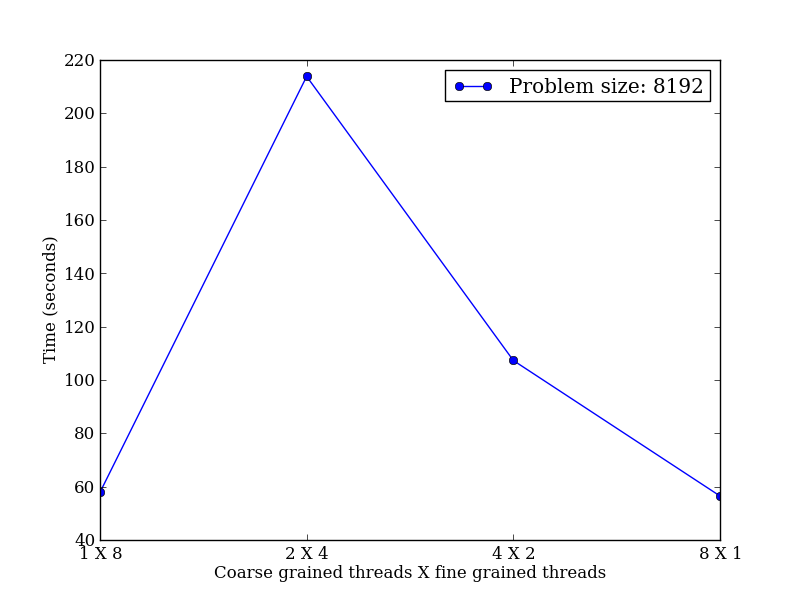
\includegraphics[width=.75\linewidth]{figures/coarse_versus_fine-grained_parallelism_(intel)}
\caption{Coarse versus fine grained parallelism}
\label{fig:combo}
\end{figure}

We also found what appears to be a bug in g++ 4.7. When scheduling only fine-grained threads in g++ compiled binaries, the running time increases drastically (Figure ~\ref{fig:combo_gcc}).

\begin{figure}[h!]
\centering
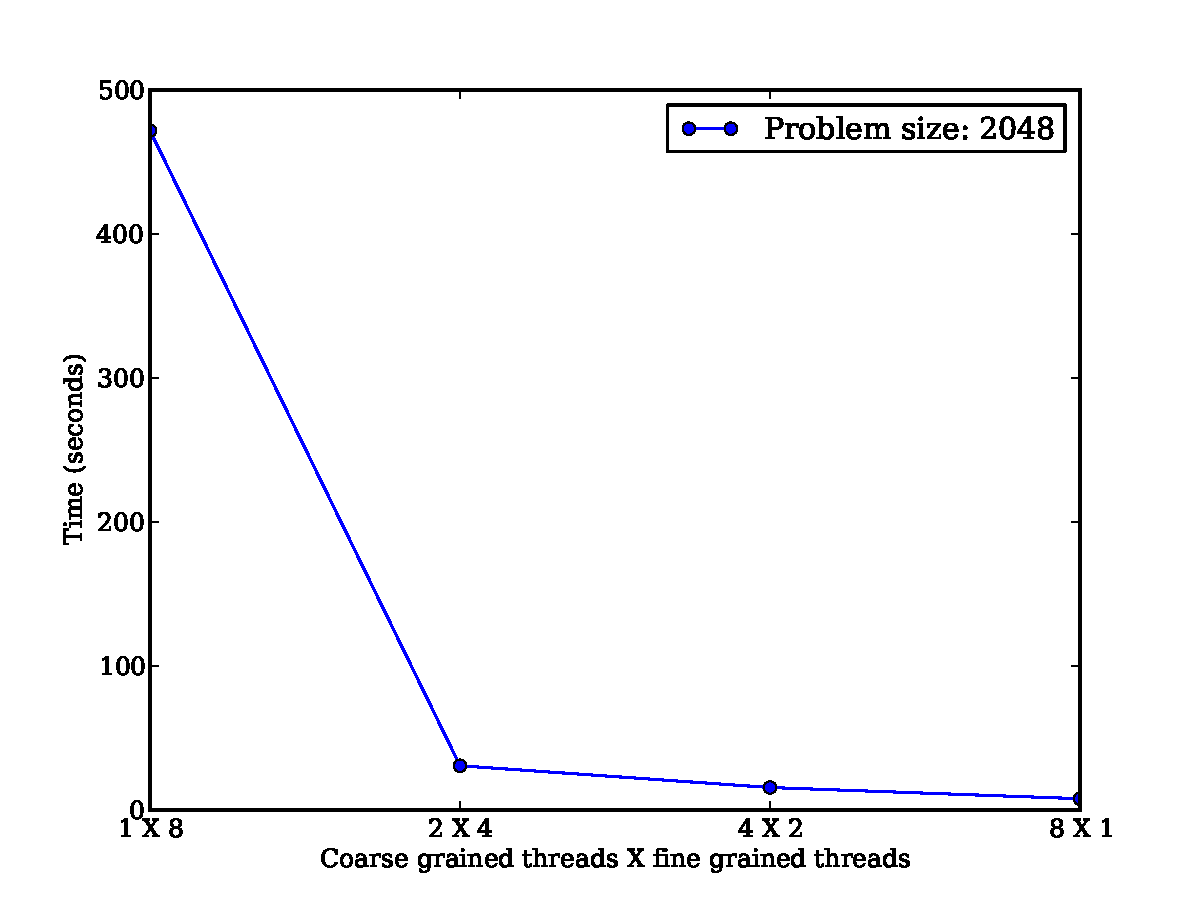
\includegraphics[width=.75\linewidth]{figures/coarse_versus_fine-grained_parallelism_(gcc)}
\caption{Coarse versus fine grained parallelism}
\label{fig:combo_gcc}
\end{figure}

If we kept the coarse-grained threads at one, but removed the outer OpenMP directive, the running time dropped to the expected amount, suggesting that the source of the bug is g++'s handling of the nested OpenMP directives. This is a relatively new feature of OpenMP that is poorly specified\footnote{\url{http://www.openmp.org/mp-documents/OpenMP4.0.0.pdf}} and saw slow adoption among the compilers. Our suspicions were further confirmed when we did not see the problematic behavior on g++ 4.8.

We were also caught off guard by how much better the GNU-compiled code performed than the Intel-compiled code. The Intel compiler, being made by the same company that manufactures the chip, is generally thought to perform better, however in our tests the GNU-compiled code ran almost twice as fast (Figure ~\ref{fig:gccvsintel}). We expect that this is a configuration issue, though we did ensure that the -O3 flag was used in all performance benchmarks.

\begin{figure}[h!]
\centering
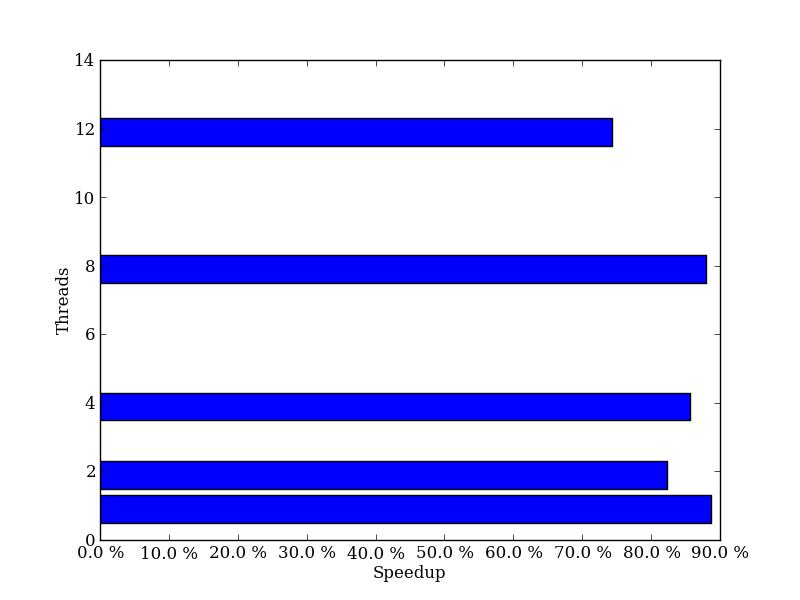
\includegraphics[width=.75\linewidth]{figures/comparison_of_intel_and_gnu_comiler_performance}
\caption{Speedup of GCC compiler over Intel compiler}
\label{fig:gccvsintel}
\end{figure}

\Section{Future Work}

Our future work would include further investigation of the poor performance we saw when combining levels of parallelism. The two approaches we would take to address this is using a version of OpenMP that supports processor affinity specification, such as the latest Intel compiler or clang-openmp\footnote{\url{http://clang-omp.github.io}}. Furthermore we could address affinity concerns by using MPI\footnote{\url{http://www.dmoz.org/Computers/Parallel_Computing/Programming/Libraries/MPI}} to create a distributed parallel system. This would also allow us to take advantage of more parallelism and decrease the time required to arrive at a solution.

\Section{Conclusion}

\begin{thebibliography}{1}
\small

\bibitem{gatech:bio}
Z. Du, Z. Yin, and D. Bader. A tile-based parallel Viterbi algorithm for biological sequence alignment on GPU with CUDA. \emph{Parallel \& Distributed Processing, Workshops and Phd Forum (IPDPSW), 2010 IEEE International Symposium on. IEEE}, 2010.

\bibitem{acs:old}
G. Fettweis, \& H. Meyr. Parallel Viterbi algorithm implementation: Breaking the ACS-bottleneck. \emph{Communications, IEEE Transactions on}, 37(8), 785-790,  1989.

%Author 1, Author 2. Title. \emph{Conference}, Year.

\end{thebibliography}

\end{document}


